
\documentclass[conference]{IEEEtran}

\usepackage{amsmath,amssymb}
\usepackage{booktabs}
\usepackage{multirow}
\usepackage{array}
\usepackage{url}
\usepackage{cite}
\usepackage{graphicx}
\usepackage{balance}
\usepackage{tikz}
\usetikzlibrary{arrows.meta,positioning,shapes.geometric,calc,fit,backgrounds}

\graphicspath{{./}{./ai/}{./ai/models/}{./models/}{./figures/}{./images/}}

\title{A Multimodal Driver Drowsiness and Distraction Monitoring System: Design and Preliminary Evaluation}

\author{
\IEEEauthorblockN{
Madhu Kunwar\IEEEauthorrefmark{1},
Madhusudan Bhandari\IEEEauthorrefmark{2},
Pranav Bhandari\IEEEauthorrefmark{3},
Samrat Giri\IEEEauthorrefmark{4}}
\IEEEauthorblockA{
Department of Software Engineering\\
Nepal College of Information Technology, zKathmandu, Nepal\\
Pokhara University\\
\IEEEauthorrefmark{1}madhu.221721@ncit.edu.np,
\IEEEauthorrefmark{2}madhusudan.221722@ncit.edu.np,
\IEEEauthorrefmark{3}pranav.221732@ncit.edu.np,
\IEEEauthorrefmark{4}samrat.221740@ncit.edu.np
}
\IEEEauthorblockA{
Supervisor: Er. Ashim Khadka\\
ashim.khadka@ncit.edu.np
}
}

\begin{document}
\maketitle

\begin{abstract}
Driver drowsiness and distraction have long been recognised as major contributors to road-traffic crashes, and low-cost driver-monitoring prototypes have frequently been restricted to a single visual cue such as eye closure. In this work, a multimodal, webcam-based driver-monitoring system has been designed and preliminarily evaluated. Five complementary visual signals---Eye Aspect Ratio (EAR), Percentage of Eye Closure (PERCLOS), Mouth Aspect Ratio (MAR), head pose, and upper-body posture---have been extracted in real time, and facial and body landmarks have been obtained using MediaPipe. The features have been normalised and combined through a transparent weighted-linear fusion model, from which a Composite Drowsiness Score has been derived and mapped to four graduated alert levels. A driver-specific calibration stage has been incorporated so that personalised baselines are established before monitoring begins. Three alert-classification configurations---a rule-based fusion system, a MobileNetV2 classifier, and a stacked ensemble---have been compared on a subject-independent split of the Driver Monitoring Dataset over 3{,}605 held-out frames. Overall accuracies of about 46\%, 57\%, and 54\% have been obtained, macro ROC-AUC values of up to 0.69 have been recorded, and an ablation study of the five cues has been reported. The most severe alert category has been found difficult to classify because of class imbalance and a face-only camera view. It has therefore been concluded that the interpretable multimodal pipeline is technically feasible, while systematic evaluation on public benchmarks has been identified as the principal remaining work.
\end{abstract}

\begin{IEEEkeywords}
driver drowsiness detection, driver distraction, Eye Aspect Ratio, PERCLOS, Mouth Aspect Ratio, head pose, posture analysis, multimodal fusion, machine learning, real-time monitoring, advanced driver assistance systems (ADAS)
\end{IEEEkeywords}

\section{Introduction}
Driving is a safety-critical task in which a momentary lapse of attention can have fatal consequences. \emph{Driver drowsiness} is a physiological state of reduced alertness caused by fatigue or sleep deprivation, in which reaction time, sustained attention, and decision-making are impaired and brief episodes of microsleep may occur. \emph{Driver distraction}, by contrast, is a diversion of attention away from the driving task towards a competing activity such as using a mobile phone, reaching for an object, or looking away from the road. Both conditions reduce the driver's capacity to respond to hazards in time, and both are therefore central concerns for road safety.

The scale of the problem is substantial. The World Health Organization has estimated road-traffic crashes to cause on the order of 1.3~million deaths each year and to rank among the foremost causes of death for young adults~\cite{who2018}. A meaningful share of these events has been linked to fatigue and inattention: official crash records attribute tens of thousands of collisions per year to drowsy driving~\cite{nhtsa}, while naturalistic studies suggest that the true involvement of drowsiness is considerably higher than police-reported figures indicate~\cite{tefft}. Because fatigue and distraction produce observable behavioural signs---slow eyelid closure, yawning, head nodding, and gaze or posture that drifts from the forward driving position---these states can, in principle, be detected before a crash occurs. This is the motivation for \emph{Driver Monitoring Systems} (DMS), which continuously observe the driver and issue a warning when the estimated state becomes unsafe~\cite{kaplan,sikander}.

Three broad families of DMS have been studied. Physiological approaches based on EEG, ECG, or electrooculography provide direct evidence of fatigue but require body-worn sensors that are intrusive and sensitive to motion~\cite{ji2004}. Vehicle-based approaches infer driver state from steering, lane keeping, and pedal behaviour, but these signals are confounded by road geometry, traffic, and driving style~\cite{baccour,mcdonald}. Camera-based (behavioural) approaches observe the driver directly and offer a practical compromise between cost, intrusiveness, and information richness, which is why they have become the dominant direction in recent low-cost systems~\cite{bergasa,ramzan}.

Most lightweight camera-only prototypes, however, depend on a \emph{single} cue. The Eye Aspect Ratio (EAR) is computationally inexpensive and effective for detecting eye closure~\cite{soukopova}, and PERCLOS extends this evidence over time~\cite{wierwille,dinges}. Yet the reliability of these ocular cues is degraded by lighting, spectacles, head rotation, and natural inter-driver differences in eye shape, and eye closure alone cannot describe distraction caused by looking away or changing posture. A system built on one hand-tuned threshold is therefore \emph{brittle}: it neither generalises across drivers nor captures the full range of unsafe behaviour.

Two design decisions follow from this observation. First, why move beyond a purely rule-based detector towards \emph{machine learning} and \emph{deep learning}? Rule-based fusion with manually chosen thresholds cannot learn the complex, non-linear appearance patterns that distinguish, for example, a phone call from safe driving, and its weights must be tuned by hand for every new condition. Learned models---a convolutional neural network (CNN) and a gradient-boosted ensemble---can instead learn such patterns from data and improve recognition of the harder, minority classes, while the interpretable rule-based system is retained for cold-start operation and transparency. Second, why adopt a \emph{multimodal} design? Because independent cues fail in different situations, combining partially uncorrelated signals---eyes, mouth, head pose, and body posture---reduces the chance that a single failure (an occluded eye, a turned head) disables the whole system and allows drowsiness and distraction to be addressed within one pipeline~\cite{du,ansari}.

From the literature, several \emph{research gaps} are identified. (i)~Many prototypes rely on a single ocular cue and cannot represent distraction. (ii)~Fixed global thresholds ignore inter-driver variability. (iii)~High-accuracy end-to-end deep models are often opaque and demand large labelled datasets and GPU hardware, which limits low-cost deployment. (iv)~Few affordable systems address drowsiness and distraction jointly. (v)~Evaluations commonly report a single accuracy figure on class-imbalanced data, hiding poor performance on the most severe states, and are seldom subject-independent~\cite{ramzan,ngxande}.

Accordingly, the \emph{objectives} of this work are: (1)~to design a single-webcam multimodal pipeline that fuses ocular, mouth, head-pose, and postural cues; (2)~to personalise decision thresholds through adaptive calibration; (3)~to produce an interpretable Composite Drowsiness Score with graduated alerts; (4)~to compare rule-based, deep-learning, and ensemble alert-classification configurations under a subject-independent protocol using confusion matrices, macro-F1, ROC-AUC, and an ablation study; and (5)~to implement the system for real-time operation on commodity hardware.

The main \emph{contributions} are:
\begin{enumerate}
    \item a single-camera multimodal pipeline that combines ocular, mouth, head-pose, and postural cues;
    \item an adaptive calibration mechanism that establishes driver-specific eye and posture baselines;
    \item an interpretable Composite Drowsiness Score with four graduated alert levels;
    \item a real-time FastAPI/WebSocket and Next.js implementation suitable for commodity hardware; and
    \item a preliminary subject-independent comparison of three alert-classification configurations, reported with per-class confusion matrices, ROC behaviour, and an ablation study rather than a single accuracy value.
\end{enumerate}

\section{Related Work}
Physiological approaches based on EEG, ECG, and electrooculography can provide direct evidence of fatigue, but the associated body-worn sensors are intrusive and prone to motion artefacts, which limits their use in ordinary vehicles~\cite{ji2004}. Vehicle-behaviour approaches use signals such as steering variation, lane position, and pedal activity; support-vector and temporal models have been applied to these signals, yet their reliability depends heavily on road and driving conditions~\cite{baccour,mcdonald}. Camera-based methods, which observe the driver directly, have therefore emerged as a practical compromise between cost, intrusiveness, and information richness, and they form the basis of most recent low-cost systems~\cite{elnabi,bergasa}.

Facial-landmark measures underpin many of these camera-based systems. The Eye Aspect Ratio was introduced as a lightweight landmark measure for real-time eye-blink detection~\cite{soukopova}, and PERCLOS, defined as the proportion of time the eyes remain closed, has been validated as a psychophysiological correlate of alertness that is better suited to sustained closure than an isolated blink~\cite{wierwille,dinges}. Yawning provides a complementary fatigue cue that can be captured with the Mouth Aspect Ratio, and the YawDD corpus has been widely used for yawn detection~\cite{abtahi}. Head pose adds information about nodding and gaze-away distraction, and landmark-based Perspective-n-Point formulations have offered a computationally practical way to recover head orientation in real time~\cite{kim,lepetit}. Reliable landmark extraction has been enabled by detectors ranging from classical cascades~\cite{viola} and regression-tree alignment~\cite{king,kazemi} to cascaded CNNs~\cite{zhang_mtcnn}; more recently, MediaPipe has provided refined 3-D face and body landmarks that run in real time on a CPU~\cite{lugaresi,bazarevsky}.

Beyond the face, upper-body posture carries information that is not always visible in facial features, and head- and body-posture models have been studied as fatigue indicators~\cite{ansari}. A large body of deep-learning work has pushed benchmark accuracy higher: transfer-learned CNN backbones such as MobileNet, ResNet, VGG, and EfficientNet~\cite{howard,sandler,he_resnet,simonyan,tan_efficientnet}, trained on ImageNet-scale data~\cite{krizhevsky,deng_imagenet}, have been fine-tuned for drowsiness, while multi-CNN, temporal, and embedded variants have targeted accuracy or deployability~\cite{ahmed,weng,florez,albadawi}. Distraction has been addressed separately through gaze and eyes-off-the-road estimation~\cite{zhang_gaze}. These learned models generally require substantial labelled data and are less interpretable, whereas multimodal fusion has been shown to improve robustness by combining partially independent signals~\cite{du}. Public datasets have supported this progress---NTHU-DDD~\cite{weng}, UTA-RLDD~\cite{ghoddoosian}, DROZY~\cite{massoz_drozy}, and, for graded distraction with video, the Driver Monitoring Dataset (DMD)~\cite{ortega_dmd}. Building on this background, the present work deliberately prioritises transparency and deployability: a rule-based weighted fusion is used as an interpretable baseline, and learned CNN and ensemble configurations~\cite{sandler,chen_xgboost} are compared against it under a subject-independent protocol.

\section{Methodology}
The system is realised as a real-time pipeline that transforms a webcam stream into a Composite Drowsiness Score and a graduated alert. Fig.~\ref{fig:pipeline} summarises the end-to-end data flow from image acquisition to the monitoring dashboard. Each stage is modular, so an individual detector or cue can be replaced or extended without redesigning the whole pipeline.

\begin{figure*}[t]
\centering
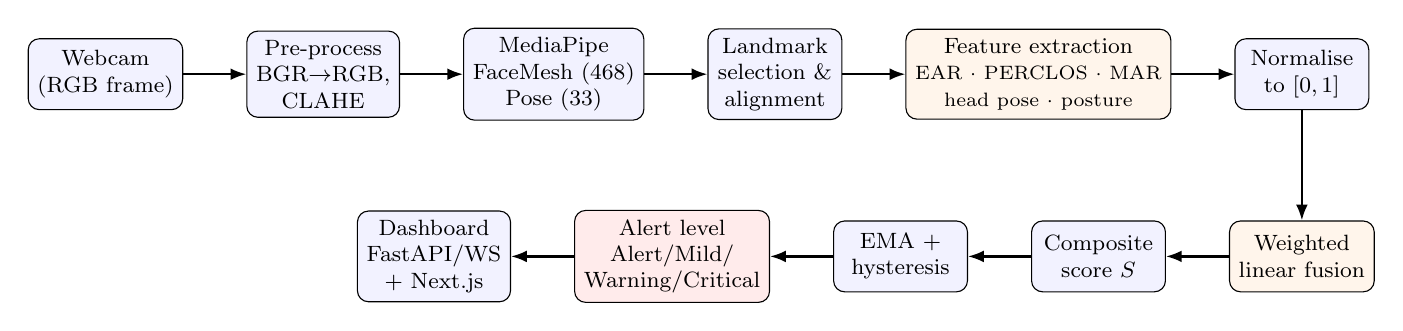
\begin{tikzpicture}[
  node distance=6mm and 8mm,
  box/.style={draw, rounded corners, align=center, minimum height=9mm, minimum width=17mm, font=\footnotesize, fill=blue!5},
  feat/.style={draw, rounded corners, align=center, minimum height=7mm, font=\scriptsize, fill=green!6},
  arr/.style={-{Latex[length=2mm]}, thick}
]
\node[box] (cam) {Webcam\\(RGB frame)};
\node[box, right=of cam] (pre) {Pre-process\\BGR$\rightarrow$RGB,\\CLAHE};
\node[box, right=of pre] (mp) {MediaPipe\\FaceMesh (468)\\Pose (33)};
\node[box, right=of mp] (align) {Landmark\\selection \&\\alignment};
\node[box, right=of align, fill=orange!8, minimum width=24mm] (fex) {Feature extraction\\{\scriptsize EAR $\cdot$ PERCLOS $\cdot$ MAR}\\{\scriptsize head pose $\cdot$ posture}};
\node[box, right=of fex] (norm) {Normalise\\to $[0,1]$};

\node[box, below=14mm of norm, fill=orange!8] (fuse) {Weighted\\linear fusion};
\node[box, left=of fuse] (score) {Composite\\score $S$};
\node[box, left=of score] (smooth) {EMA +\\hysteresis};
\node[box, left=of smooth, fill=red!8] (level) {Alert level\\Alert/Mild/\\Warning/Critical};
\node[box, left=of level] (dash) {Dashboard\\FastAPI/WS\\+ Next.js};

\draw[arr] (cam) -- (pre);
\draw[arr] (pre) -- (mp);
\draw[arr] (mp) -- (align);
\draw[arr] (align) -- (fex);
\draw[arr] (fex) -- (norm);
\draw[arr] (norm) -- (fuse);
\draw[arr] (fuse) -- (score);
\draw[arr] (score) -- (smooth);
\draw[arr] (smooth) -- (level);
\draw[arr] (level) -- (dash);
\end{tikzpicture}
\caption{End-to-end methodology. Webcam frames are pre-processed, landmarks are extracted with MediaPipe FaceMesh and Pose, five cues are computed and normalised, and a weighted-linear fusion produces a Composite Drowsiness Score that---after temporal smoothing---is mapped to one of four graduated alert levels and streamed to the dashboard.}
\label{fig:pipeline}
\end{figure*}

\subsection{Landmark Acquisition and Calibration}
OpenCV~\cite{bradski} captures each frame and converts it from BGR to RGB, and contrast-limited adaptive histogram equalisation is applied in low light. MediaPipe FaceMesh then provides 468 facial landmarks and MediaPipe Pose provides 33 body landmarks~\cite{lugaresi,bazarevsky}. If no face is detected, feature computation is skipped for that frame while the session continues. During the first $\approx$30 frames, an adaptive calibration window records the driver's open-eye EAR statistics and upright-posture baseline, so that personalised rather than global thresholds are used thereafter.

\subsection{Eye Aspect Ratio and PERCLOS}
For the six landmarks around an eye (Fig.~\ref{fig:eye}), the EAR is defined as
\begin{equation}
EAR = \frac{\lVert p_2-p_6\rVert+\lVert p_3-p_5\rVert}{2\,\lVert p_1-p_4\rVert}.
\end{equation}
The left- and right-eye values are averaged. During calibration the mean $\mu_{EAR}$ and standard deviation $\sigma_{EAR}$ of the open-eye ratio are estimated, and an adaptive closure threshold is set as
\begin{equation}
\tau_{eye}=\mu_{EAR}-k\,\sigma_{EAR},
\end{equation}
which removes the dependence on one fixed threshold for all drivers. PERCLOS is then the proportion of frames in a rolling window for which the eye is closed:
\begin{equation}
PERCLOS=\frac{\#\{t:\,EAR_t<\tau_{eye}\}}{N}\times100\%.
\end{equation}
Because an ordinary blink occupies only a few frames, PERCLOS remains low for brief blinks and rises only when closure persists.

\begin{figure}[t]
\centering
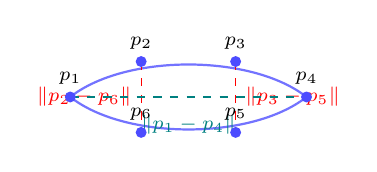
\begin{tikzpicture}[scale=1.0,
  lm/.style={circle, fill=blue!70, inner sep=1.4pt},
  lbl/.style={font=\scriptsize}]
% eye contour points p1..p6 (open eye almond shape)
\coordinate (p1) at (0.0,0.0);
\coordinate (p2) at (0.9,0.45);
\coordinate (p3) at (2.1,0.45);
\coordinate (p4) at (3.0,0.0);
\coordinate (p5) at (2.1,-0.45);
\coordinate (p6) at (0.9,-0.45);
\draw[thick,blue!55] (p1) .. controls (0.7,0.55) and (2.3,0.55) .. (p4)
                     .. controls (2.3,-0.55) and (0.7,-0.55) .. (p1);
% vertical distances
\draw[dashed,red] (p2)--(p6) node[midway,left,lbl]{$\lVert p_2-p_6\rVert$};
\draw[dashed,red] (p3)--(p5) node[midway,right,lbl]{$\lVert p_3-p_5\rVert$};
\draw[dashed,teal] (p1)--(p4) node[midway,below=3pt,lbl]{$\lVert p_1-p_4\rVert$};
\foreach \p/\n in {p1/$p_1$,p2/$p_2$,p3/$p_3$,p4/$p_4$,p5/$p_5$,p6/$p_6$}{
  \node[lm] at (\p){}; \node[lbl,above=1pt] at (\p){\n};}
\end{tikzpicture}
\caption{Six eye landmarks used for EAR. The two vertical distances (red) shrink as the eyelid closes, while the horizontal distance (teal) stays roughly constant, so the ratio falls sharply during eye closure.}
\label{fig:eye}
\end{figure}

\subsection{Mouth Aspect Ratio}
The MAR is computed from eight mouth landmarks (Fig.~\ref{fig:mouth}):
\begin{equation}
MAR=\frac{\lVert p_2-p_8\rVert+\lVert p_3-p_7\rVert+\lVert p_4-p_6\rVert}{2\,\lVert p_1-p_5\rVert}.
\end{equation}
A sustained increase above a calibrated threshold is treated as evidence of yawning, rather than reacting to a single wide-mouth frame.

\begin{figure}[t]
\centering
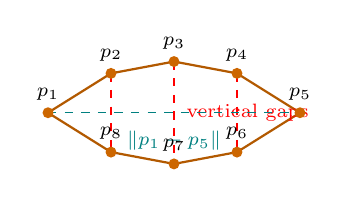
\begin{tikzpicture}[scale=1.0,
  lm/.style={circle, fill=orange!80!black, inner sep=1.4pt},
  lbl/.style={font=\scriptsize}]
% mouth (open) points p1..p8
\coordinate (p1) at (0.0,0.0);   % left corner
\coordinate (p2) at (0.8,0.5);
\coordinate (p3) at (1.6,0.65);
\coordinate (p4) at (2.4,0.5);
\coordinate (p5) at (3.2,0.0);   % right corner
\coordinate (p6) at (2.4,-0.5);
\coordinate (p7) at (1.6,-0.65);
\coordinate (p8) at (0.8,-0.5);
\draw[thick,orange!70!black] (p1)--(p2)--(p3)--(p4)--(p5)--(p6)--(p7)--(p8)--cycle;
\draw[dashed,red] (p2)--(p8);
\draw[dashed,red] (p3)--(p7) node[midway,right=1pt,lbl]{vertical gaps};
\draw[dashed,red] (p4)--(p6);
\draw[dashed,teal] (p1)--(p5) node[midway,below=3pt,lbl]{$\lVert p_1-p_5\rVert$};
\foreach \p/\n in {p1/$p_1$,p2/$p_2$,p3/$p_3$,p4/$p_4$,p5/$p_5$,p6/$p_6$,p7/$p_7$,p8/$p_8$}{
  \node[lm] at (\p){}; \node[lbl,above=1pt] at (\p){\n};}
\end{tikzpicture}
\caption{Eight mouth landmarks used for MAR. The three vertical lip gaps (red) grow during a yawn while the mouth width (teal) changes little, so a sustained rise in the ratio indicates yawning.}
\label{fig:mouth}
\end{figure}

\subsection{Head Pose and Posture}
Head-pose angles (pitch, yaw, and roll) are recovered from six selected facial landmarks and a canonical 3-D face model using a Perspective-n-Point formulation~\cite{lepetit}. Sustained downward pitch is interpreted as a nodding cue, and excessive yaw is treated as evidence of looking away from the road. Posture is estimated from MediaPipe Pose shoulder and nose landmarks: the calibration stage fixes an upright baseline from the shoulder vector and the nose offset, and the posture score is the normalised deviation from this baseline, capturing forward slouching and lateral lean.

\subsection{Feature Fusion and Alert Logic}
Each of the five raw features is mapped to a normalised contribution $f\in[0,1]$, and the Composite Drowsiness Score is formed as a weighted linear combination:
\begin{equation}
S = 0.30f_{EAR}+0.25f_{PER}+0.20f_{MAR}+0.15f_{head}+0.10f_{pos}.
\end{equation}
The weights sum to one and give the greatest influence to ocular evidence while retaining complementary information from yawning, head orientation, and posture. To avoid alarms that flicker frame-to-frame, $S$ is passed through an exponential moving average ($\alpha=0.3$) and the alert \emph{level} uses hysteresis, so escalation and de-escalation require the smoothed score to cross different bounds. The four graduated levels and their responses are given in Table~\ref{tab:thresholds}; the same four class names---Alert, Mild, Warning, and Critical---are used consistently throughout the paper and in the evaluation, so that the operating levels and the confusion-matrix classes coincide.

\begin{table}[t]
\caption{Composite-score thresholds and graduated alert responses}
\label{tab:thresholds}
\centering
\begin{tabular}{ccl}
\toprule
Composite score $S$ & Alert level & System response\\
\midrule
$S<0.25$            & Alert    & Silent monitoring\\
$0.25\leq S<0.50$   & Mild     & Visual caution\\
$0.50\leq S<0.75$   & Warning  & Warning + soft audio\\
$S\geq0.75$         & Critical & Urgent repeating alarm\\
\bottomrule
\end{tabular}
\end{table}

\section{Implementation}
The prototype uses OpenCV for video acquisition and geometric processing~\cite{bradski}, MediaPipe FaceMesh and Pose for landmark extraction~\cite{lugaresi}, and NumPy for numerical operations~\cite{harris_numpy}. The backend is a FastAPI service that exchanges frames and state over a WebSocket, and the browser dashboard is built with Next.js. No dedicated physiological sensors, vehicle-bus integration, or remote fleet backend is required. The dashboard shows a live video panel with landmarks, five feature gauges, a composite-score gauge, and an alert banner, all driven from the same WebSocket state so that displayed values and the alert level stay synchronised. The learned classifiers are served through ONNX Runtime so that the server remains lightweight; the exported MobileNetV2 model is 9.6~MB and its measured inference latency is about 1.0~ms (p50) to 1.3~ms (p95) per frame. The system targets $\approx$30~frames/s on a conventional laptop, and manual testing showed continuous dashboard updates without noticeable interruption.

\section{Experimental Setup}
Two forms of evaluation were carried out. First, controlled functional tests examined whether each visual cue responded to the behaviour it was designed to represent. Second, three alert-classification configurations were compared: System~A, the rule-based weighted fusion of the five cues; System~B, a MobileNetV2 CNN fine-tuned from ImageNet weights on face crops; and System~C, an XGBoost stacked ensemble~\cite{chen_xgboost} that combines System~A's signals with System~B's class probabilities. The learned models were trained with class weighting and data augmentation and optimised with Adam~\cite{kingma}.

The configurations were evaluated on the Driver Monitoring Dataset (DMD)~\cite{ortega_dmd}, whose per-frame OpenLABEL action labels were mapped to the four alert levels (Alert, Mild, Warning, Critical). A \emph{subject-independent} split was used---training, validation, and test groups contain different drivers---so that generalisation to unseen people is tested rather than memorisation. The held-out test set contains 3{,}605 frames with class counts of 1{,}997 (Alert), 821 (Mild), 525 (Warning), and 262 (Critical), so the set is markedly imbalanced. Because of this imbalance, performance is reported with per-class confusion matrices, macro-averaged precision, recall and F1, and one-vs-rest ROC-AUC, rather than with overall accuracy alone.

\section{Results and Discussion}
The confusion matrices for the three configurations are given in Table~\ref{tab:cm}, and their summary metrics in Table~\ref{tab:summary}. Overall diagonal agreement was about 46\% for System~A, 57\% for System~B, and 54\% for System~C. These headline figures, however, conceal strongly class-dependent behaviour. System~B attains the highest accuracy by predicting the majority Alert class almost exclusively---1{,}972 of 1{,}997 Alert frames are recovered, but only 80 of 821 Mild, 10 of 525 Warning, and none of the Critical frames---so its accuracy is largely a reflection of class imbalance and its macro-F1 (0.23) is the lowest of the three. System~C spreads its predictions across Alert and Mild and, as a result, achieves the best macro-recall (0.34) and macro-F1 (0.31) despite a lower raw accuracy than System~B. The interpretable System~A, which was designed around drowsiness cues, is at a disadvantage on these distraction labels yet still yields a macro-F1 comparable to the much larger CNN. A consistent and important observation is that the Critical class is essentially never predicted by any configuration: it is both the rarest class (262 frames) and, being a hand-based texting/reaching behaviour, is only weakly observable from a face-only view. This resolves the apparent gap between a high overall number and true multi-class competence and directly motivates class-aware reporting.

\begin{table}[t]
\caption{Confusion matrices on the 3{,}605-frame subject-independent test set (rows: true class; columns: predicted). Diagonal entries are shown in bold.}
\label{tab:cm}
\centering
\footnotesize
\setlength{\tabcolsep}{4pt}

\textbf{System A (rule-based fusion)}\\[2pt]
\begin{tabular}{lcccc}
\toprule
True\,$\backslash$\,Pred & Alert & Mild & Warning & Critical\\
\midrule
Alert    & \textbf{1329} & 636 & 32 & 0\\
Mild     & 491 & \textbf{323} & 7 & 0\\
Warning  & 176 & 337 & \textbf{12} & 0\\
Critical & 136 & 121 & 5 & \textbf{0}\\
\bottomrule
\end{tabular}\\[6pt]

\textbf{System B (MobileNetV2)}\\[2pt]
\begin{tabular}{lcccc}
\toprule
True\,$\backslash$\,Pred & Alert & Mild & Warning & Critical\\
\midrule
Alert    & \textbf{1972} & 22 & 3 & 0\\
Mild     & 731 & \textbf{80} & 10 & 0\\
Warning  & 498 & 17 & \textbf{10} & 0\\
Critical & 239 & 18 & 5 & \textbf{0}\\
\bottomrule
\end{tabular}\\[6pt]

\textbf{System C (stacked ensemble)}\\[2pt]
\begin{tabular}{lcccc}
\toprule
True\,$\backslash$\,Pred & Alert & Mild & Warning & Critical\\
\midrule
Alert    & \textbf{1442} & 534 & 21 & 0\\
Mild     & 322 & \textbf{486} & 13 & 0\\
Warning  & 99 & 397 & \textbf{27} & 2\\
Critical & 80 & 171 & 11 & \textbf{0}\\
\bottomrule
\end{tabular}
\end{table}

\begin{figure*}[t]
\centering
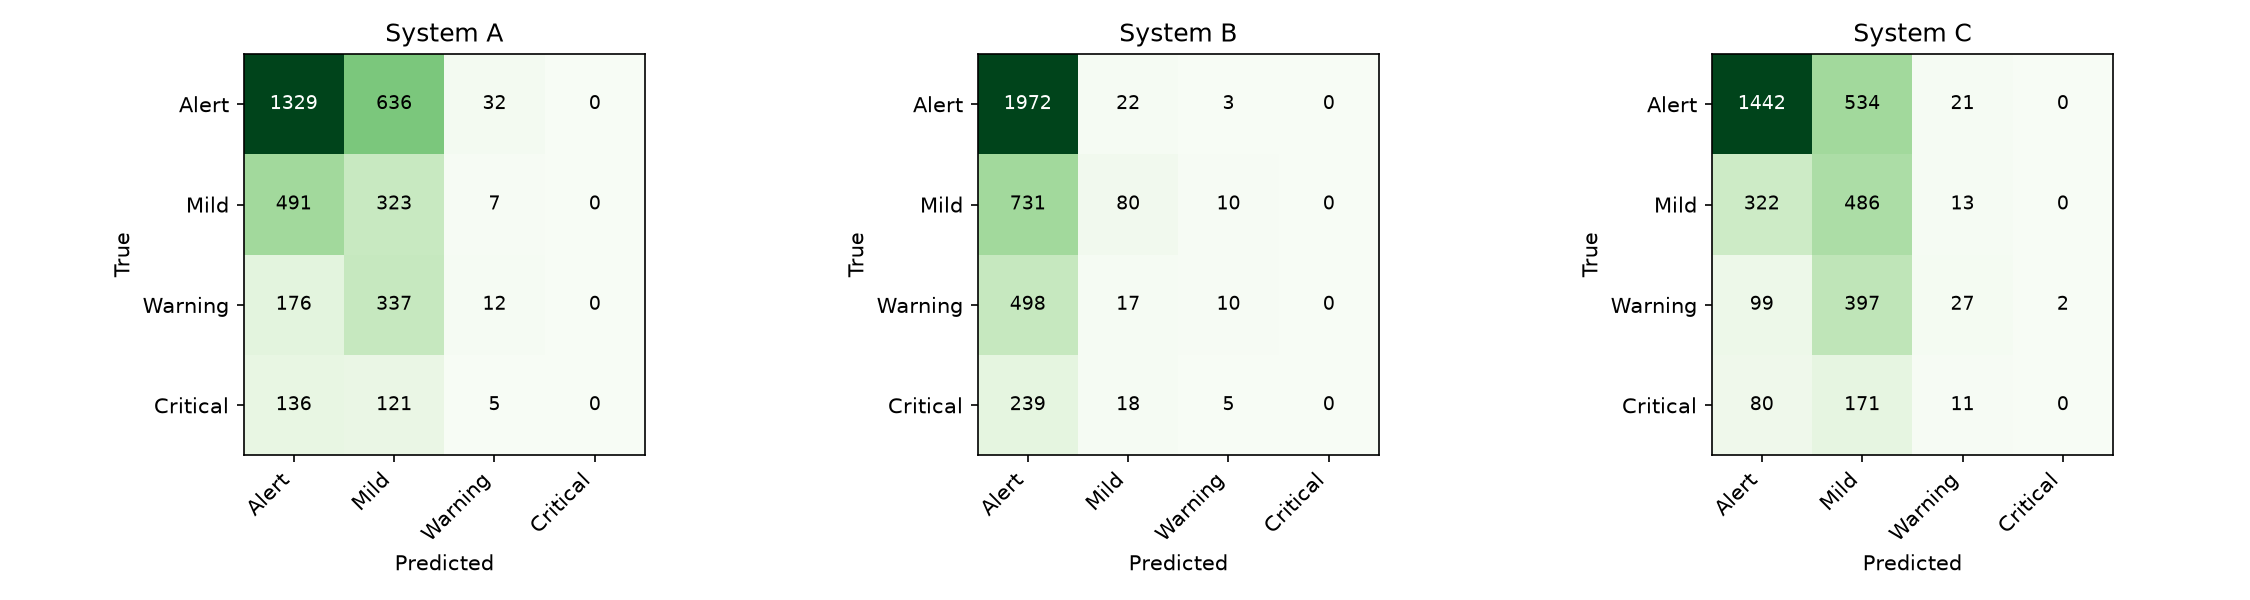
\includegraphics[width=0.92\textwidth]{confusion_matrices.png}
\caption{Confusion-matrix heat maps for the three candidate alert-classification configurations (System~A: rule-based; System~B: MobileNetV2; System~C: ensemble) on the 3{,}605-frame subject-independent test set. The cell counts correspond to Table~\ref{tab:cm}.}
\label{fig:cm}
\end{figure*}

\begin{table}[t]
\caption{Summary metrics for the three configurations (macro-averaged)}
\label{tab:summary}
\centering
\begin{tabular}{lcccc}
\toprule
System & Accuracy & Precision & Recall & F1\\
\midrule
A --- rule-based    & 46.2\% & 26.6\% & 27.0\% & 24.3\%\\
B --- MobileNetV2   & \textbf{57.2\%} & 37.9\% & 27.6\% & 23.2\%\\
C --- ensemble      & 54.2\% & 35.6\% & \textbf{34.1\%} & \textbf{30.7\%}\\
\bottomrule
\end{tabular}
\end{table}

One-vs-rest ROC analysis was performed for the two learned configurations, which expose a continuous decision score; System~A's fixed-threshold rule does not, so it was excluded from this comparison. The resulting curves are shown in Fig.~\ref{fig:roc}. System~B obtained AUCs of 0.71 (Alert), 0.64 (Mild), 0.71 (Warning), and 0.62 (Critical), for a macro AUC of 0.67, while System~C obtained 0.75, 0.63, 0.77, and 0.60 respectively, for a macro AUC of 0.69. Every value exceeds the 0.5 chance level, which indicates that the learned models do carry genuine discriminative signal for each class even where their thresholded predictions collapse onto the majority class; the low Critical recall is therefore largely a threshold and imbalance effect rather than a complete absence of signal. The separation between lower and elevated states is clearly easier than distinguishing the most severe category, which argues for class-balanced training and threshold calibration in future work.

\begin{figure}[t]
\centering
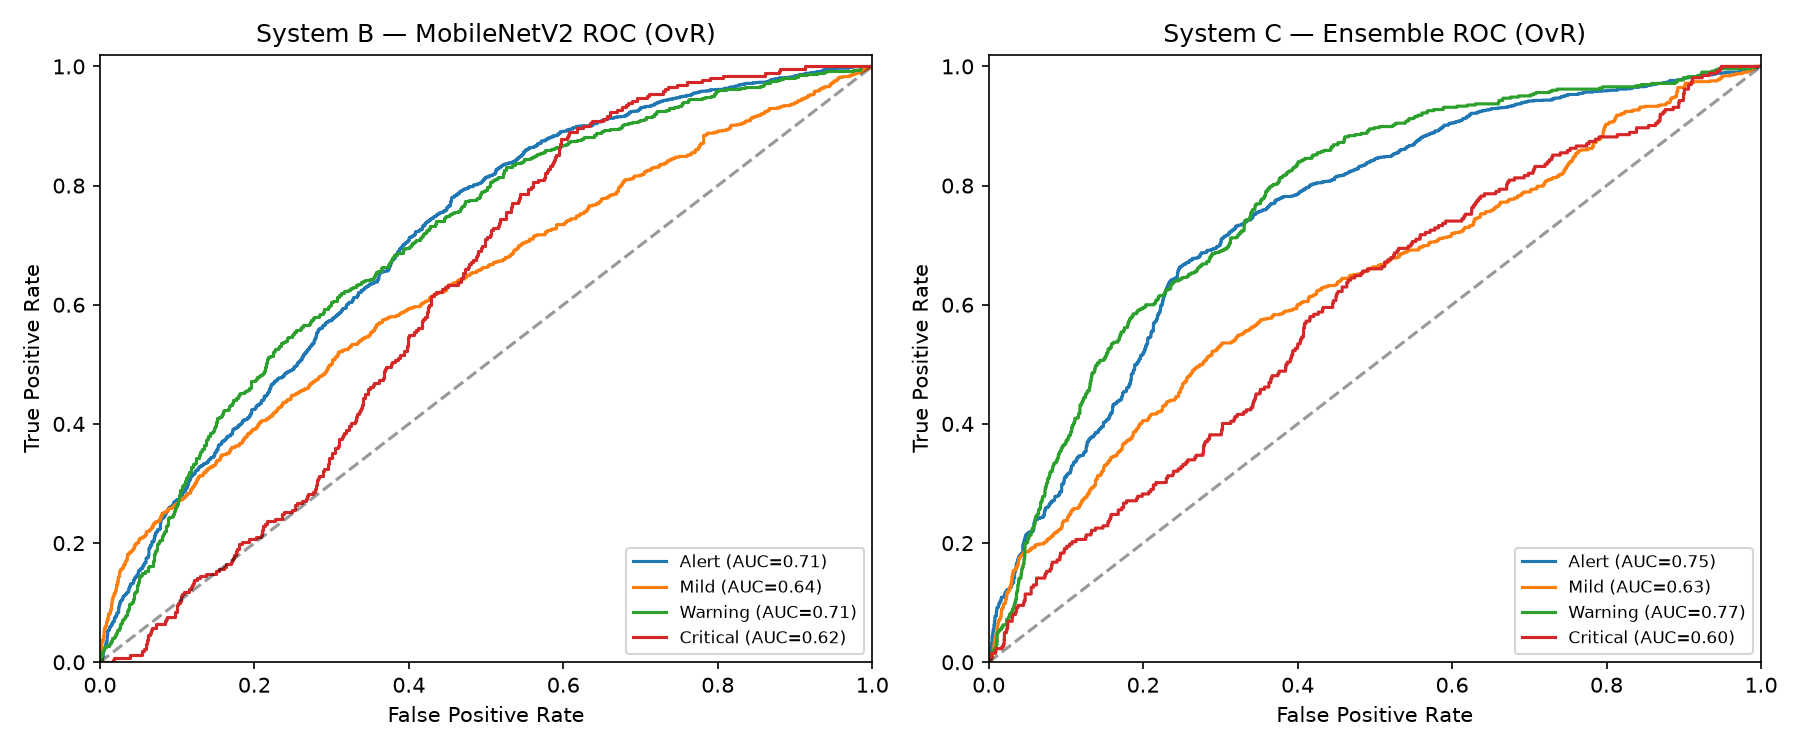
\includegraphics[width=\columnwidth]{roc_curves.png}
\caption{One-vs-rest ROC curves for System~B (MobileNetV2) and System~C (ensemble) across the four alert categories. All curves lie above the chance diagonal.}
\label{fig:roc}
\end{figure}

An ablation study over the five cues of System~A is reported in Table~\ref{tab:ablation} and visualised in Fig.~\ref{fig:ablation}. As cues are added, raw accuracy falls (53.7\% for EAR-only to 46.2\% for all five) while macro-F1 improves (20.1\% to 24.3\%). This behaviour is expected and informative: the DMD test labels describe \emph{distraction}, so adding drowsiness-oriented cues shifts predictions away from the dominant Alert class and trades majority-class accuracy for more balanced multi-class recognition. The ablation confirms that each cue contributes to the balanced metric rather than being redundant, and it explains why the rule-based system, though weaker on raw accuracy, remains a useful and interpretable component.

\begin{table}[t]
\caption{Ablation of System~A cues (macro-averaged, DMD test set)}
\label{tab:ablation}
\centering
\begin{tabular}{lcccc}
\toprule
Cue set & Accuracy & Precision & Recall & F1\\
\midrule
EAR only              & 53.7\% & 26.3\% & 25.5\% & 20.1\%\\
+ PERCLOS             & 53.4\% & 19.4\% & 24.6\% & 18.7\%\\
+ MAR                 & 50.4\% & 23.7\% & 24.1\% & 20.2\%\\
+ Head pose           & 45.6\% & 26.0\% & 27.7\% & 24.9\%\\
+ Posture (all five)  & 46.2\% & 26.6\% & 27.0\% & 24.3\%\\
\bottomrule
\end{tabular}
\end{table}

\begin{figure}[t]
\centering
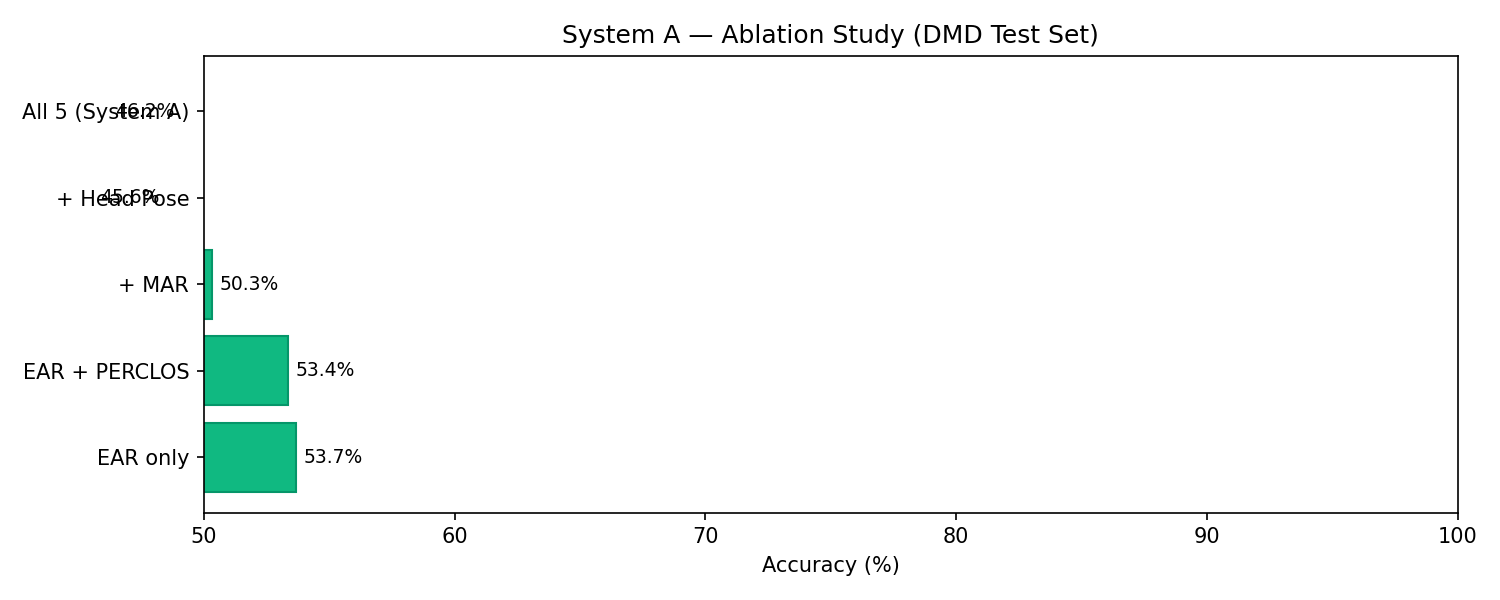
\includegraphics[width=\columnwidth]{ablation_study.png}
\caption{Ablation study: effect of progressively adding cues to System~A on accuracy and macro-averaged precision, recall, and F1. Values correspond to Table~\ref{tab:ablation}.}
\label{fig:ablation}
\end{figure}

The controlled functional tests showed the expected responses of the individual cues. EAR decreased sharply during eye closure, PERCLOS stayed low for ordinary short blinks and rose during sustained closure, and MAR increased during prolonged mouth opening and returned to baseline afterwards. Head-pose estimation tracked sustained downward pitch during nodding but showed more frame-to-frame variation under partial landmark occlusion. The posture signal behaved as designed, though its baseline remained sensitive to driver height, seating, and camera placement, and it is therefore treated as implemented but not yet fully validated.

Taken together, the results support the technical feasibility of a transparent multimodal pipeline rather than establishing deployment-level accuracy. The principal benefit of the approach is interpretability: every contribution to the score can be inspected, and each alert can be traced to measurable visual cues, which is valuable for debugging, threshold calibration, and safety justification. Several limitations remain. RGB vision degrades in low light and strong backlighting; spectacles, occlusion, and extreme head rotation reduce landmark quality; the fusion weights were chosen from the literature rather than optimised on labelled data; the face-only view caps recognition of hand-based distraction; and the three-driver split, while genuinely subject-independent, is small. These limitations frame the future work below.

\section{Conclusion and Future Work}
A multimodal driver drowsiness and distraction detection prototype based on a single RGB webcam has been presented. Five complementary cues---EAR, PERCLOS, MAR, head pose, and upper-body posture---have been extracted with MediaPipe and OpenCV and combined through a transparent weighted-linear fusion model, and an adaptive calibration stage together with four graduated alert levels has supported driver-specific, temporally stable monitoring. Real-time operation on commodity hardware has been demonstrated, and three alert-classification configurations have been compared under a subject-independent protocol over 3{,}605 held-out frames.

Accuracies of about 46\%, 57\%, and 54\% have been obtained for the rule-based, MobileNetV2, and ensemble configurations, but the per-class confusion matrices, an ablation study, and one-vs-rest ROC-AUC (up to 0.69 macro) have shown that these headline numbers are dominated by class imbalance and a face-only view. In particular, the ensemble has achieved the most balanced recognition, while the most severe category has remained difficult for every configuration. These findings have been interpreted as evidence of feasibility and as a justification for reporting class-aware metrics rather than accuracy alone; they are not claimed as benchmark-level performance.

Future work will proceed in four directions. First, posture calibration will be completed across seating positions and camera placements, followed by data-driven optimisation of the fusion weights. Second, the complete system will be evaluated on public benchmarks such as NTHU-DDD, YawDD, and DMD using accuracy, precision, recall, F1, balanced accuracy, ROC-AUC, frame rate, and latency, with additional drivers and hand-camera views to lift severe-class recall. Third, robustness will be tested under low light, eyewear, occlusion, and head-pose variation. Finally, the learned fusion classifier will be wired into the live decision and compared directly with the interpretable rule-based fusion.

\begin{thebibliography}{50}

\bibitem{who2018}
World Health Organization, \emph{Global Status Report on Road Safety 2018}. Geneva: WHO, 2018.

\bibitem{nhtsa}
National Highway Traffic Safety Administration, ``Drowsy driving,'' \emph{Traffic Safety Facts}, NHTSA, Washington, DC, 2017.

\bibitem{tefft}
B. C. Tefft, ``Prevalence of motor vehicle crashes involving drowsy drivers, United States, 2009--2013,'' AAA Foundation for Traffic Safety, Washington, DC, Tech. Rep., 2014.

\bibitem{kaplan}
S. Kaplan, M. A. Guvensan, A. G. Yavuz, and Y. Karalurt, ``Driver behavior analysis for safe driving: A survey,'' \emph{IEEE Trans. Intell. Transp. Syst.}, vol. 16, no. 6, pp. 3017--3032, 2015.

\bibitem{sikander}
G. Sikander and S. Anwar, ``Driver fatigue detection systems: A review,'' \emph{IEEE Trans. Intell. Transp. Syst.}, vol. 20, no. 6, pp. 2339--2352, 2019.

\bibitem{ji2004}
Q. Ji, Z. Zhu, and P. Lan, ``Real-time nonintrusive monitoring and prediction of driver fatigue,'' \emph{IEEE Trans. Veh. Technol.}, vol. 53, no. 4, pp. 1052--1068, 2004.

\bibitem{baccour}
M. H. Baccour, F. Driewer, T. Sch\"ack, and E. Kasneci, ``Comparative analysis of vehicle-based and driver-based features for driver drowsiness monitoring by support vector machines,'' \emph{IEEE Trans. Intell. Transp. Syst.}, vol. 23, no. 12, pp. 23164--23178, 2022.

\bibitem{mcdonald}
A. D. McDonald, C. Schwarz, J. D. Lee, and T. L. Brown, ``A contextual and temporal algorithm for driver drowsiness detection,'' \emph{Accident Analysis \& Prevention}, vol. 113, pp. 25--37, 2018.

\bibitem{bergasa}
L. M. Bergasa, J. Nuevo, M. A. Sotelo, R. Barea, and M. E. Lopez, ``Real-time system for monitoring driver vigilance,'' \emph{IEEE Trans. Intell. Transp. Syst.}, vol. 7, no. 1, pp. 63--77, 2006.

\bibitem{ramzan}
M. Ramzan, H. U. Khan, S. M. Awan, A. Ismail, M. Ilyas, and A. Mahmood, ``A survey on state-of-the-art drowsiness detection techniques,'' \emph{IEEE Access}, vol. 7, pp. 61904--61919, 2019.

\bibitem{ngxande}
M. Ngxande, J.-R. Tapamo, and M. Burke, ``Driver drowsiness detection using behavioral measures and machine learning techniques: A review of state-of-art techniques,'' in \emph{Proc. PRASA-RobMech Int. Conf.}, 2017, pp. 156--161.

\bibitem{elnabi}
S. A. El-Nabi, W. El-Shafai, E.-S. M. El-Rabaie, K. F. Ramadan, F. E. Abd El-Samie, and S. Mohsen, ``Machine learning and deep learning techniques for driver fatigue and drowsiness detection: A review,'' \emph{Multimedia Tools and Applications}, vol. 83, no. 3, pp. 9441--9477, 2023.

\bibitem{soukopova}
T. Soukupov\'a and J. \v{C}ech, ``Real-time eye blink detection using facial landmarks,'' in \emph{Proc. 21st Computer Vision Winter Workshop (CVWW)}, Rimske Toplice, Slovenia, 2016.

\bibitem{wierwille}
W. W. Wierwille and L. A. Ellsworth, ``Evaluation of driver drowsiness by trained raters,'' \emph{Accident Analysis \& Prevention}, vol. 26, no. 5, pp. 571--581, 1994.

\bibitem{dinges}
D. F. Dinges and R. Grace, ``PERCLOS: A valid psychophysiological measure of alertness as assessed by psychomotor vigilance,'' Federal Highway Administration, Tech. Rep. FHWA-MCRT-98-006, 1998.

\bibitem{abtahi}
S. Abtahi, M. Omidyeganeh, S. Shirmohammadi, and B. Hariri, ``YawDD: A yawning detection dataset,'' in \emph{Proc. 5th ACM Multimedia Systems Conf.}, 2014, pp. 24--28.

\bibitem{kim}
D. Kim, H. Park, T. Kim, W. Kim, and J. Paik, ``Real-time driver monitoring system with facial landmark-based eye closure detection and head pose recognition,'' \emph{Scientific Reports}, vol. 13, p. 18264, 2023.

\bibitem{lepetit}
V. Lepetit, F. Moreno-Noguer, and P. Fua, ``EPnP: An accurate $O(n)$ solution to the PnP problem,'' \emph{Int. J. Computer Vision}, vol. 81, no. 2, pp. 155--166, 2009.

\bibitem{viola}
P. Viola and M. Jones, ``Rapid object detection using a boosted cascade of simple features,'' in \emph{Proc. IEEE CVPR}, 2001, pp. I-511--I-518.

\bibitem{king}
D. E. King, ``Dlib-ml: A machine learning toolkit,'' \emph{J. Machine Learning Research}, vol. 10, pp. 1755--1758, 2009.

\bibitem{kazemi}
V. Kazemi and J. Sullivan, ``One millisecond face alignment with an ensemble of regression trees,'' in \emph{Proc. IEEE CVPR}, 2014, pp. 1867--1874.

\bibitem{zhang_mtcnn}
K. Zhang, Z. Zhang, Z. Li, and Y. Qiao, ``Joint face detection and alignment using multitask cascaded convolutional networks,'' \emph{IEEE Signal Processing Letters}, vol. 23, no. 10, pp. 1499--1503, 2016.

\bibitem{lugaresi}
C. Lugaresi \emph{et al.}, ``MediaPipe: A framework for building perception pipelines,'' arXiv:1906.08172, 2019.

\bibitem{bazarevsky}
V. Bazarevsky, I. Grishchenko, K. Raveendran, T. Zhu, F. Zhang, and M. Grundmann, ``BlazePose: On-device real-time body pose tracking,'' arXiv:2006.10204, 2020.

\bibitem{ansari}
S. Ansari, F. Naghdy, H. Du, and Y. N. Pahnwar, ``Driver mental fatigue detection based on head posture using new modified ReLU-BiLSTM deep neural network,'' \emph{IEEE Trans. Intell. Transp. Syst.}, vol. 23, no. 8, pp. 10957--10969, 2022.

\bibitem{du}
G. Du \emph{et al.}, ``A multimodal fusion fatigue driving detection method based on heart rate and PERCLOS,'' \emph{IEEE Trans. Intell. Transp. Syst.}, vol. 23, no. 11, pp. 21810--21820, 2022.

\bibitem{howard}
A. G. Howard \emph{et al.}, ``MobileNets: Efficient convolutional neural networks for mobile vision applications,'' arXiv:1704.04861, 2017.

\bibitem{sandler}
M. Sandler, A. Howard, M. Zhu, A. Zhmoginov, and L.-C. Chen, ``MobileNetV2: Inverted residuals and linear bottlenecks,'' in \emph{Proc. IEEE CVPR}, 2018, pp. 4510--4520.

\bibitem{he_resnet}
K. He, X. Zhang, S. Ren, and J. Sun, ``Deep residual learning for image recognition,'' in \emph{Proc. IEEE CVPR}, 2016, pp. 770--778.

\bibitem{simonyan}
K. Simonyan and A. Zisserman, ``Very deep convolutional networks for large-scale image recognition,'' in \emph{Proc. Int. Conf. Learning Representations (ICLR)}, 2015.

\bibitem{tan_efficientnet}
M. Tan and Q. Le, ``EfficientNet: Rethinking model scaling for convolutional neural networks,'' in \emph{Proc. Int. Conf. Machine Learning (ICML)}, 2019, pp. 6105--6114.

\bibitem{krizhevsky}
A. Krizhevsky, I. Sutskever, and G. E. Hinton, ``ImageNet classification with deep convolutional neural networks,'' in \emph{Advances in Neural Information Processing Systems (NeurIPS)}, 2012, pp. 1097--1105.

\bibitem{deng_imagenet}
J. Deng, W. Dong, R. Socher, L.-J. Li, K. Li, and L. Fei-Fei, ``ImageNet: A large-scale hierarchical image database,'' in \emph{Proc. IEEE CVPR}, 2009, pp. 248--255.

\bibitem{chen_xgboost}
T. Chen and C. Guestrin, ``XGBoost: A scalable tree boosting system,'' in \emph{Proc. 22nd ACM SIGKDD Int. Conf. Knowledge Discovery and Data Mining}, 2016, pp. 785--794.

\bibitem{kingma}
D. P. Kingma and J. Ba, ``Adam: A method for stochastic optimization,'' in \emph{Proc. Int. Conf. Learning Representations (ICLR)}, 2015.

\bibitem{ahmed}
M. Ahmed, S. Masood, M. Ahmad, and A. A. Abd El-Latif, ``Intelligent driver drowsiness detection for traffic safety based on multi CNN deep model and facial subsampling,'' \emph{IEEE Trans. Intell. Transp. Syst.}, vol. 23, no. 10, pp. 19743--19752, 2022.

\bibitem{weng}
C.-H. Weng, Y.-H. Lai, and S.-H. Lai, ``Driver drowsiness detection via a hierarchical temporal deep belief network,'' in \emph{Computer Vision -- ACCV 2016 Workshops}, Part III, 2017, pp. 117--133.

\bibitem{florez}
R. Florez, F. Palomino-Quispe, A. B. Alvarez, R. J. Coaquira-Castillo, and J. C. Herrera-Levano, ``A real-time embedded system for driver drowsiness detection based on visual analysis of the eyes and mouth using convolutional neural network and mouth aspect ratio,'' \emph{Sensors}, vol. 24, no. 19, p. 6261, 2024.

\bibitem{albadawi}
Y. Albadawi, A. AlRedhaei, and M. Takruri, ``Real-time machine learning-based driver drowsiness detection using visual features,'' \emph{Journal of Imaging}, vol. 9, no. 5, p. 91, 2023.

\bibitem{zhang_gaze}
X. Zhang, Y. Sugano, M. Fritz, and A. Bulling, ``Appearance-based gaze estimation in the wild,'' in \emph{Proc. IEEE CVPR}, 2015, pp. 4511--4520.

\bibitem{ortega_dmd}
J. D. Ortega \emph{et al.}, ``DMD: A large-scale multi-modal driver monitoring dataset for attention and alertness analysis,'' in \emph{Computer Vision -- ECCV 2020 Workshops}, 2020, pp. 387--405.

\bibitem{ghoddoosian}
R. Ghoddoosian, M. Galib, and V. Athitsos, ``A realistic dataset and baseline temporal model for early drowsiness detection,'' in \emph{Proc. IEEE CVPR Workshops}, 2019, pp. 178--187.

\bibitem{massoz_drozy}
Q. Massoz, T. Langohr, C. Fran\c{c}ois, and J. G. Verly, ``The ULg multimodality drowsiness database (DROZY) and examples of use,'' in \emph{Proc. IEEE Winter Conf. Applications of Computer Vision (WACV)}, 2016, pp. 1--7.

\bibitem{bradski}
G. Bradski, ``The OpenCV library,'' \emph{Dr. Dobb's Journal of Software Tools}, vol. 25, no. 11, pp. 120--125, 2000.

\bibitem{harris_numpy}
C. R. Harris \emph{et al.}, ``Array programming with NumPy,'' \emph{Nature}, vol. 585, pp. 357--362, 2020.

\end{thebibliography}

\balance
\end{document}
